\documentclass{article}


% if you need to pass options to natbib, use, e.g.:
%     \PassOptionsToPackage{numbers, compress}{natbib}
% before loading neurips_2024


% ready for submission
\usepackage[preprint]{neurips_2024}


% to compile a preprint version, e.g., for submission to arXiv, add add the
% [preprint] option:
%     \usepackage[preprint]{neurips_2024}


% to compile a camera-ready version, add the [final] option, e.g.:
%     \usepackage[final]{neurips_2024}


% to avoid loading the natbib package, add option nonatbib:
%    \usepackage[nonatbib]{neurips_2024}


\usepackage[utf8]{inputenc} % allow utf-8 input
\usepackage[T1]{fontenc}    % use 8-bit T1 fonts
\usepackage{hyperref}       % hyperlinks
\usepackage{url}            % simple URL typesetting
\usepackage{booktabs}       % professional-quality tables
\usepackage{amsfonts}       % blackboard math symbols
\usepackage{nicefrac}       % compact symbols for 1/2, etc.
\usepackage{microtype}      % microtypography
\usepackage{xcolor}         % colors
\usepackage{pifont}
\usepackage{graphicx}
\usepackage{float}


\title{Documentation of Bit Sequence mini RL project}


% The \author macro works with any number of authors. There are two commands
% used to separate the names and addresses of multiple authors: \And and \AND.
%
% Using \And between authors leaves it to LaTeX to determine where to break the
% lines. Using \AND forces a line break at that point. So, if LaTeX puts 3 of 4
% authors names on the first line, and the last on the second line, try using
% \AND instead of \And before the third author name.


\author{%
  Chau Yu Hei\thanks{Currently not a student yet :(} \\
  HKUST\\
  20644747\\
  \texttt{yhchau@connect.ust.hk} \\
  % examples of more authors
  % \And
  % Coauthor \\
  % Affiliation \\
  % Address \\
  % \texttt{email} \\
  % \AND
  % Coauthor \\
  % Affiliation \\
  % Address \\
  % \texttt{email} \\
  % \And
  % Coauthor \\
  % Affiliation \\
  % Address \\
  % \texttt{email} \\
  % \And
  % Coauthor \\
  % Affiliation \\
  % Address \\
  % \texttt{email} \\
}


\begin{document}


\maketitle


\begin{abstract}
GFlowNets provide a new paradigm for finetuning LLMs with respect to some energy function. However, a common problem is that strings with high probability are often very rare compared to the strings with low probability. How do we efficiently tune LLMs using the GFlowNet algorithm so that it is able to learn from sparse rewards? In this mini-project, we attempt to tackle the problem of generating a randomly prechosen bit string using old RL methods.
\end{abstract}


\section{Background}
Recent work has shown that GFlowNets are able to generate diverse samples for LLMs, and finetune LLMs according to Bayesian updates (\cite{hu_llm}). However, their experiments are limited to generating text sequences of short length. How do we generate text sequences of larger lengths? It is evident that most strings have low reward due to the large search space of the set of all possible text sequences.

In this mini-project, we attempt to tackle a similar toy problem, that is, to generate a specific bit sequence in the set of all bit sequences. We first apply a naive DQN method for sequence generation, and show that the method only works for small $n$. Then we attempt to apply Hindsight Experience Replay (HER) (\cite{hindsight_openai}) by OpenAI to see whether the method successfully generates the correct bit sequences for longer sequence lengths.

\section{Problem setting}
Here we attempt to use a DQN to generate a predesignated randomly picked target bit sequence. In each setting, an integer $1 \leq n \leq 50$ is fixed, and the state space is $\mathcal{S}_n=\{0,1\}^n$. If we make the graph complete by allowing full $2^n$ actions for every transition, the DQN will be too expensive in memory to parameterize (since we need to compute $\max$ over the action space). So we consider the actions to be flipping a bit $\mathcal{A}_n=\{i \in \mathbb{Z}|0 \leq i \leq n-1\}$ (using computer indexing convention). 

The goal is to find a policy $\pi: (s,g)  \in \mathcal{S}_n \times \mathcal{S}_n \mapsto \pi(s,g) \in \mathcal{A}_n$ such that the agent is able to start from $s$ and arrive at the goal $g \in \mathcal{S}_n$ in the least amount of steps. To this end, we train a goal conditioned DQN $(s,g,a) \mapsto Q_g(s,a) \in \mathbb{R}$. The reward function $R(s,g,a)=1$ iff the next state $s \rightarrow_a s' = g$, and would be $0$ otherwise.

The intuition is that, for low values of $n$ (maybe $1 \leq n \leq 10$?), a naive DQN is able to learn to arrive at the bit sequence due to exhausting the search space (along with using the parallel processing by GPUs). However, for large values of $n$, this would be infeasible, since the reward is too sparse.


\section{Experiments}
In the below experiments, we run vanilla-DQN and HER-DQN with $n=5,10,15,20,30,40,50$. We test two kinds of network architectures, namely UVFA (\cite{UVFA}), and a Handcrafted ARchitecture (HAR) that has strong inductive bias towards the bitflipping state-action space. Please refer to the Appendix \ref{appendix} for more details on the network architectures. \\

The agent will perform at most $n$ steps in each episode. For all experiments, we run 16 agents simultaneously for training episodes, while 1024 agents will be run simultaneously for testing episodes. We only modify the replay buffer during the training episodes, while the testing episodes do not alter the replay buffer. The replay buffer has a maximum $2^{15}$ capacity, and previous experiences will be sampled from the buffer uniformly during replay (optimizing $Q$ network). All other relevant hyperparameters (such as lr, $\gamma$, etc) are kept the same for each experiment. \\

The starting state $s \in \mathcal{S}_n$ and target $g \in \mathcal{S}_n$ for each 16 agents (resp. 1024) are initialized randomly and uniformly. The agents follow a $\epsilon$-probability random exploration chance starting from $\epsilon=1.0$ and decaying to $\epsilon=0.1$ with exponential decay factor $0.999$. To save time, we run at most 3000 episodes for each experiment. Assuming the states explored are uniformly random, we expect on average approximately $16 \times n \times 3000 = 48000n$ states to be explored during training, which is dominated by $|\mathcal{S}_n|=2^n$ for large $n$.

As expected, vanilla DQN with UVFA is unable to learn the optimal policy for $n=15,20$ since the probability of getting the reward is too sparse ($\frac{48000n}{2^n} << 1$). The DQN mostly sees $0$ all the time as the reward, and as a result unable to learn anything useful. If we use the handcrafted architecture (HAR), vanilla DQN is able to learn for $n=20$ due to strong inductive bias towards the bitflipping problem. However, it fails for $n=30,40,50$ (Table \ref{table1}). 

In contrast, HER-DQN with UVFA succeeds on all $n=5,10,15$, and with HAR succeeds on all $n=20,30,40,50$. Although HER-DQN fails for $n=20$ (UVFA), the success rate and mean distance to target are improving much more rapidly as compared to vanilla-DQN with UVFA on $n=20$ (see \ref{figure}). This shows the superiority of HER-DQN.

By experimenting with a handcrafted architecture with strong inductive bias towards bitflipping state-action space, we dispel the possibility that an inappropriate architecture or optimization difficulty causes vanilla-DQN to fail on high $n$, the only reason that could be is that vanilla-DQN is prone to sparse rewards. 

For detailed code on the experiments, please refer to \href{https://github.com/louis845/BitSeqRLToyProblem}{the Github repo}. For more details on the experiment setup, and some miscellaneous challenges faced and tricks used, please refer to the appendix. For other visualizations and graphs, please refer to \href{https://github.com/louis845/BitSeqRLToyProblem/blob/main/bitflipping_dqn_target_implementation.ipynb}{Vanilla-DQN notebook} \href{https://github.com/louis845/BitSeqRLToyProblem/blob/main/bitflipping_dqn_target_her_implementation.ipynb}{HER-DQN notebook} in GitHub. For further discussions and research motivated by this, please refer to \href{https://github.com/louis845/BitSeqRLToyProblemPrivateDocs/blob/master/docs/docs.pdf}{(private documentation)} or email. 

\begin{table}
  \caption{DQN experiments (max 3000 episodes)}
  \label{table1}
  \centering
  \begin{tabular}{cccccccc}
\cline{2-8}
             & \multicolumn{7}{c}{$n=$}                                                                                                                                                                                 \\ \cline{2-8} 
             & 5                          & 10                         & 15                         & 20                         & 30                         & 40                         & 50                         \\ \hline
HER-UVFA     & \ding{51} & \ding{51} & \ding{51} & \ding{55} & ?                          & ?                          & ?                          \\ \hline
Vanilla-UVFA & \ding{51} & \ding{51} & \ding{55} & \ding{55} & ?                          & ?                          & ?                          \\ \hline
HER-HAR      & ?                          & ?                          & ?                          & \ding{51} & \ding{51} & \ding{51} & \ding{51} \\ \hline
Vanilla-HAR  & ?                          & ?                          & ?                          & \ding{51} & \ding{55} & \ding{55} & \ding{55} \\ \hline
\end{tabular} \\
	\phantom{e}\\
	\ding{51}: Converged to 1.00 success rate \\
	\ding{55}: Failed to converge to 1.00 success rate \\
	?: Didn't run
\end{table}

\bibliographystyle{plainnat}
\bibliography{citations}

\clearpage
\section{Appendix}\label{appendix}
\subsection{Details for $n=20$}
\begin{figure}[H]\label{figure}
  \centering
  \fbox{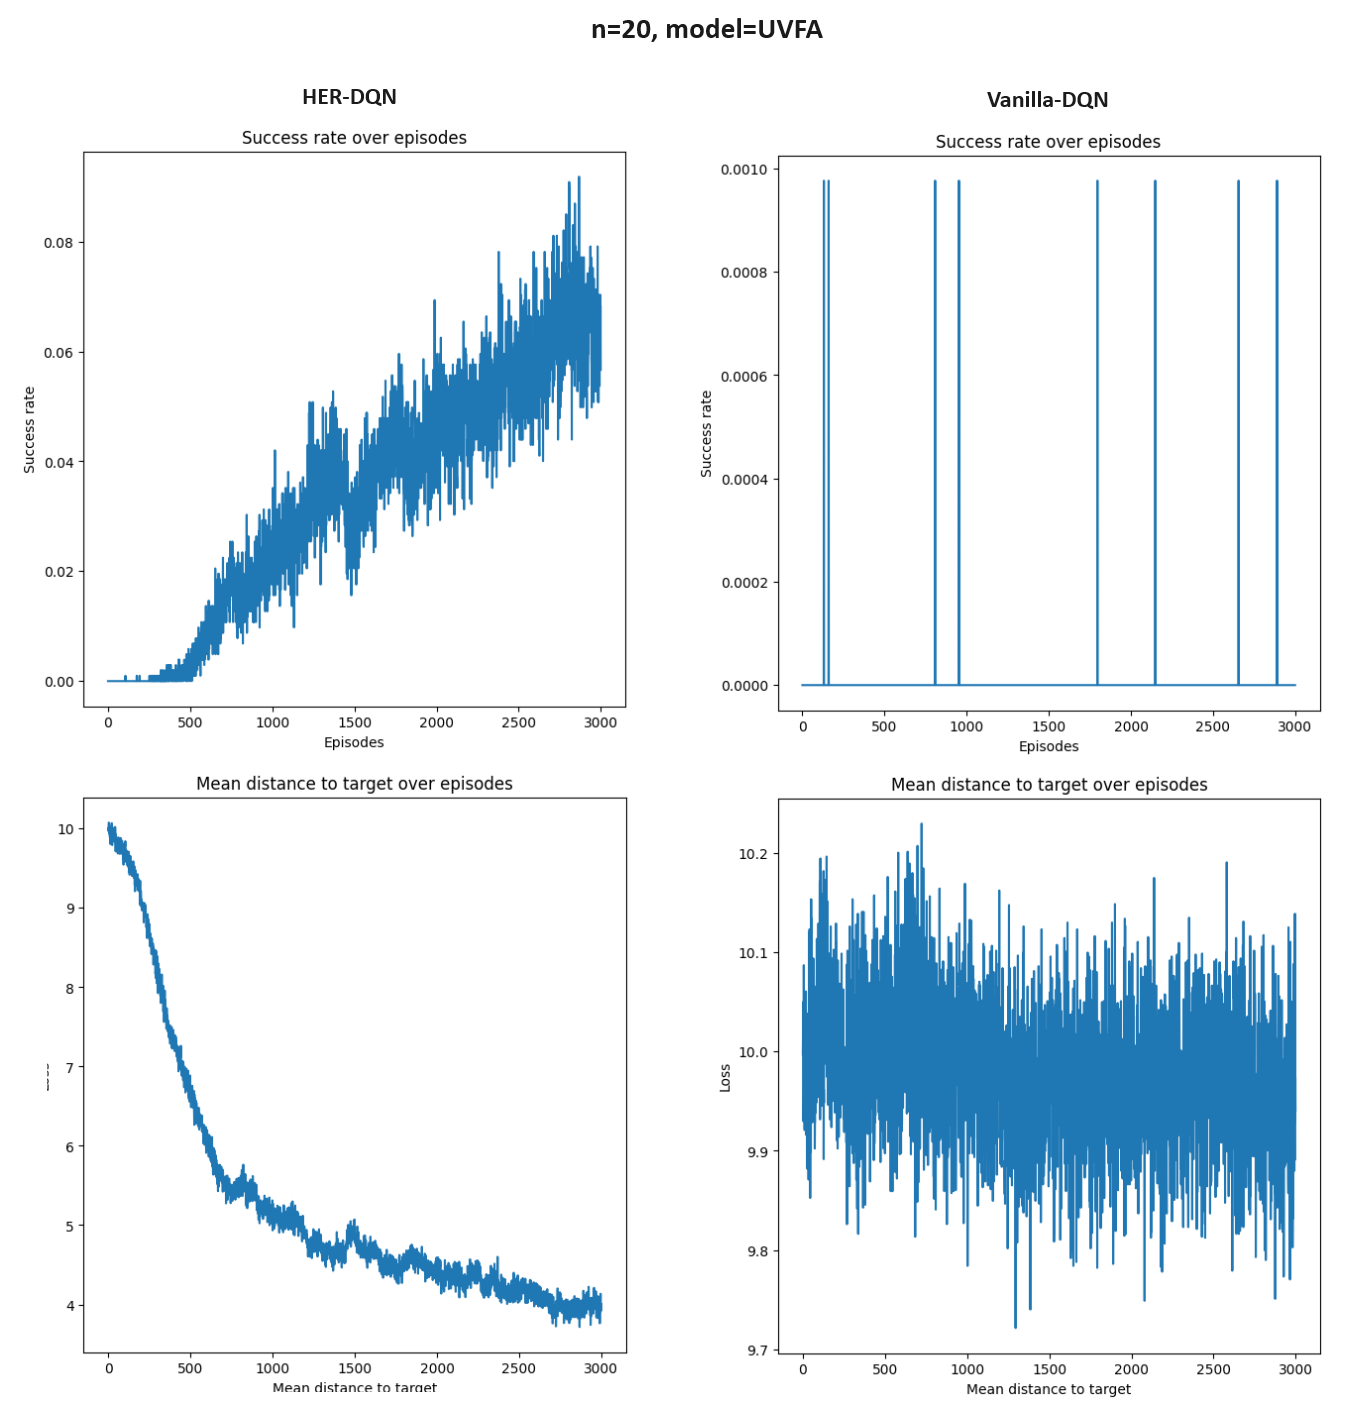
\includegraphics[scale=0.4]{image.png}}
  \caption{Metrics for $n=20$}
\end{figure}
\subsection{Network architectures}
For UVFA \cite{UVFA}, the authors recommend learning the states and goals in the same latent space and using a simple dot product as the $Q$-value. It is well-known that pre-composing linear transforms before dot product is equivalent to a bilinear operation. Therefore, we simply use a single nn.Linear layer following by GELU activation to map the state and goal to $\mathbb{R}^{128}$ vectors, and use a learnable bilinear form $\mathbb{R}^{128} \otimes \mathbb{R}^{128} \rightarrow \mathbb{R}^n$. \\

For the Handcrafted ARchitecture (HAR), it is intuitive that whether to flip the bit at $i$ depends only on $\|s-g\|_1$ and $|s[i]-g[i]|$. We therefore parameterize $Q_g(s,a)=\phi_\theta(\|s-g\|_1,|s[a]-g[a]|)$ where $\phi_\theta: \mathbb{R}^2 \rightarrow \mathbb{R}$ is a neural network with parameters $\theta$. Formally, we can define an equivalence relation $\sim$ on $\mathcal{S}_n \times \mathcal{S}_n$ invariant to permutation of the bits, and note that the optimal $Q^*(s,g,a)$ factors through $\sim$. So this is like acting on the quotient space of the original state-goal-action space (which has less elements). 
\subsection{Poylak averaging trick}
Initially, I tried to fit the DQN directly using Bellman's equation. However, the training loss is unstable and blows up occasionally, which makes the training dynamics quite noisy. After a lot of debugging, I searched online and usually people use Polyak averaging trick to separate the policy network and target network, where the target network's weights are updated slower than the policy network weights by exponential averaging. \\

Let $\theta, \phi$ be the weights of the $Q_{policy}$ and $Q_{target}$. Initially, we set $\theta=\phi$. During optimization, we compute $\theta \leftarrow \theta + lr * \frac{dL}{d\theta}$, and afterwards update $\phi \leftarrow 0.99\phi + 0.01 \theta$. So $Q_\phi$ will update slower compared to $Q_\theta$. Note that the actual update step for $\theta$ is the Adam optimizer algorithm instead of simple SGD.
\subsection{Target clipping trick}
After solving the noisy updates problem, another problem emerged where the loss somehow keeps increasing for large $n$ (irrespective of network architecture and whether HER is used). Note that this is worse when HER is present. After some debugging, the source of this problem is due to the update $Q_{policy}(s,g,a) = R_g(s,a) + \gamma \max_a Q_{target}(s,g,a)$. In my experiments, I picked a relatively large $\gamma$ close to $1$ (or else the rewards will be too small when $n=50$). 

Assuming that $Q_{policy}(s,g,a),Q_{target}(s,g,a)$ approximately follows the same distribution over the space $\mathcal{S}_n \times \mathcal{S}_n \times \mathcal{A}_n$ (since the target is an averaged version of policy), we intuitively have $E_{s,g,a}[Q_{policy}(s,g,a)] < E_{s,g}[\max_a Q_{target}(s,g,a)]$ since there is maximum in the target. If the increase is larger than $\gamma$ in the optimization trajectory $\theta_1,\theta_2,\theta_3,\cdots$, then it is expected that the $Q$-values explode to infinity.

This also explains why this phenomenon is much worse when HER is present. With HER, much more saved experiences have $R_g(s,a)=1$ (since HER biases the distribution in the replay buffer to having more rewards with non-zero values). 

To tackle this problem, we note that the actual target for an optimal $Q^*$ is in $[0,1]$, since the termination states are at $s=g$, which gives reward $1$, and other states have
$$Q^*(s,g,a) = \underbrace{R_g(s,a)}_{=0} + \gamma \underbrace{\max_a Q^*(s,g,a)}_{\leq 1}$$
by induction. By clipping the target values in $[0,1]$, the training loss is stabilized. 
\end{document}